 \documentclass[10pt, letterpaper, answer]{exam}
\usepackage{graphicx, amsmath, tikz}   
\usepackage[margin=1in]{geometry}
\usetikzlibrary{decorations.pathreplacing} 

\usepackage[breakable]{tcolorbox}
\usepackage{parskip} 
\usepackage[outputdir=../]{minted}

%%% Comment this out to remove answer boxes.
\printanswers

\title{Math 215 El Ni\~no Southern Oscillations Homework}

\author{Nathan Bailey, Sven Bachmann, and Peter Harrington}

\date{}

\setlength{\arrayrulewidth}{0.25mm}
\setlength{\tabcolsep}{18pt}
\renewcommand{\arraystretch}{2}

% PACKAGES NECESSARY FOR SYZYGY CODE BELOW

    



\usepackage[breakable]{tcolorbox}
    \usepackage{parskip} % Stop auto-indenting (to mimic markdown behaviour)
    

    % Basic figure setup, for now with no caption control since it's done
    % automatically by Pandoc (which extracts ![](path) syntax from Markdown).
    \usepackage{graphicx}
    % Maintain compatibility with old templates. Remove in nbconvert 6.0
    \let\Oldincludegraphics\includegraphics
    \usepackage{float}
    \floatplacement{figure}{H} % forces figures to be placed at the correct location
    \usepackage{xcolor} % Allow colors to be defined
    \usepackage{enumerate} % Needed for markdown enumerations to work
    \usepackage{geometry} % Used to adjust the document margins
    \usepackage{amsmath} % Equations
    \usepackage{amssymb} % Equations
    \usepackage{textcomp} % defines textquotesingle
    % Hack from http://tex.stackexchange.com/a/47451/13684:
    \AtBeginDocument{%
        \def\PYZsq{\textquotesingle}% Upright quotes in Pygmentized code
    }
    \usepackage{upquote} % Upright quotes for verbatim code
    \usepackage{eurosym} % defines \euro

    \usepackage{iftex}
    \ifPDFTeX
        \usepackage[T1]{fontenc}
        \IfFileExists{alphabeta.sty}{
              \usepackage{alphabeta}
          }{
              \usepackage[mathletters]{ucs}
              \usepackage[utf8x]{inputenc}
          }
    \else
        \usepackage{fontspec}
        \usepackage{unicode-math}
    \fi

    \usepackage{fancyvrb} % verbatim replacement that allows latex
    \usepackage{grffile} % extends the file name processing of package graphics
                         % to support a larger range
    \makeatletter % fix for old versions of grffile with XeLaTeX
    \@ifpackagelater{grffile}{2019/11/01}
    {
      % Do nothing on new versions
    }
    {
      \def\Gread@@xetex#1{%
        \IfFileExists{"\Gin@base".bb}%
        {\Gread@eps{\Gin@base.bb}}%
        {\Gread@@xetex@aux#1}%
      }
    }
    \makeatother
    \usepackage[Export]{adjustbox} % Used to constrain images to a maximum size
    \adjustboxset{max size={0.9\linewidth}{0.9\paperheight}}

    % The hyperref package gives us a pdf with properly built
    % internal navigation ('pdf bookmarks' for the table of contents,
    % internal cross-reference links, web links for URLs, etc.)
    \usepackage{hyperref}
    % The default LaTeX title has an obnoxious amount of whitespace. By default,
    % titling removes some of it. It also provides customization options.
    \usepackage{titling}
    \usepackage{longtable} % longtable support required by pandoc >1.10
    \usepackage{booktabs}  % table support for pandoc > 1.12.2
    \usepackage{array}     % table support for pandoc >= 2.11.3
    \usepackage{calc}      % table minipage width calculation for pandoc >= 2.11.1
    \usepackage[inline]{enumitem} % IRkernel/repr support (it uses the enumerate* environment)
    \usepackage[normalem]{ulem} % ulem is needed to support strikethroughs (\sout)
                                % normalem makes italics be italics, not underlines
    \usepackage{soul}      % strikethrough (\st) support for pandoc >= 3.0.0
    \usepackage{mathrsfs}
    

    
    % Colors for the hyperref package
    \definecolor{urlcolor}{rgb}{0,.145,.698}
    \definecolor{linkcolor}{rgb}{.71,0.21,0.01}
    \definecolor{citecolor}{rgb}{.12,.54,.11}

    % ANSI colors
    \definecolor{ansi-black}{HTML}{3E424D}
    \definecolor{ansi-black-intense}{HTML}{282C36}
    \definecolor{ansi-red}{HTML}{E75C58}
    \definecolor{ansi-red-intense}{HTML}{B22B31}
    \definecolor{ansi-green}{HTML}{00A250}
    \definecolor{ansi-green-intense}{HTML}{007427}
    \definecolor{ansi-yellow}{HTML}{DDB62B}
    \definecolor{ansi-yellow-intense}{HTML}{B27D12}
    \definecolor{ansi-blue}{HTML}{208FFB}
    \definecolor{ansi-blue-intense}{HTML}{0065CA}
    \definecolor{ansi-magenta}{HTML}{D160C4}
    \definecolor{ansi-magenta-intense}{HTML}{A03196}
    \definecolor{ansi-cyan}{HTML}{60C6C8}
    \definecolor{ansi-cyan-intense}{HTML}{258F8F}
    \definecolor{ansi-white}{HTML}{C5C1B4}
    \definecolor{ansi-white-intense}{HTML}{A1A6B2}
    \definecolor{ansi-default-inverse-fg}{HTML}{FFFFFF}
    \definecolor{ansi-default-inverse-bg}{HTML}{000000}

    % common color for the border for error outputs.
    \definecolor{outerrorbackground}{HTML}{FFDFDF}

    % commands and environments needed by pandoc snippets
    % extracted from the output of `pandoc -s`
    \providecommand{\tightlist}{%
      \setlength{\itemsep}{0pt}\setlength{\parskip}{0pt}}
    \DefineVerbatimEnvironment{Highlighting}{Verbatim}{commandchars=\\\{\}}
    % Add ',fontsize=\small' for more characters per line
    \newenvironment{Shaded}{}{}
    \newcommand{\KeywordTok}[1]{\textcolor[rgb]{0.00,0.44,0.13}{\textbf{{#1}}}}
    \newcommand{\DataTypeTok}[1]{\textcolor[rgb]{0.56,0.13,0.00}{{#1}}}
    \newcommand{\DecValTok}[1]{\textcolor[rgb]{0.25,0.63,0.44}{{#1}}}
    \newcommand{\BaseNTok}[1]{\textcolor[rgb]{0.25,0.63,0.44}{{#1}}}
    \newcommand{\FloatTok}[1]{\textcolor[rgb]{0.25,0.63,0.44}{{#1}}}
    \newcommand{\CharTok}[1]{\textcolor[rgb]{0.25,0.44,0.63}{{#1}}}
    \newcommand{\StringTok}[1]{\textcolor[rgb]{0.25,0.44,0.63}{{#1}}}
    \newcommand{\CommentTok}[1]{\textcolor[rgb]{0.38,0.63,0.69}{\textit{{#1}}}}
    \newcommand{\OtherTok}[1]{\textcolor[rgb]{0.00,0.44,0.13}{{#1}}}
    \newcommand{\AlertTok}[1]{\textcolor[rgb]{1.00,0.00,0.00}{\textbf{{#1}}}}
    \newcommand{\FunctionTok}[1]{\textcolor[rgb]{0.02,0.16,0.49}{{#1}}}
    \newcommand{\RegionMarkerTok}[1]{{#1}}
    \newcommand{\ErrorTok}[1]{\textcolor[rgb]{1.00,0.00,0.00}{\textbf{{#1}}}}
    \newcommand{\NormalTok}[1]{{#1}}

    % Additional commands for more recent versions of Pandoc
    \newcommand{\ConstantTok}[1]{\textcolor[rgb]{0.53,0.00,0.00}{{#1}}}
    \newcommand{\SpecialCharTok}[1]{\textcolor[rgb]{0.25,0.44,0.63}{{#1}}}
    \newcommand{\VerbatimStringTok}[1]{\textcolor[rgb]{0.25,0.44,0.63}{{#1}}}
    \newcommand{\SpecialStringTok}[1]{\textcolor[rgb]{0.73,0.40,0.53}{{#1}}}
    \newcommand{\ImportTok}[1]{{#1}}
    \newcommand{\DocumentationTok}[1]{\textcolor[rgb]{0.73,0.13,0.13}{\textit{{#1}}}}
    \newcommand{\AnnotationTok}[1]{\textcolor[rgb]{0.38,0.63,0.69}{\textbf{\textit{{#1}}}}}
    \newcommand{\CommentVarTok}[1]{\textcolor[rgb]{0.38,0.63,0.69}{\textbf{\textit{{#1}}}}}
    \newcommand{\VariableTok}[1]{\textcolor[rgb]{0.10,0.09,0.49}{{#1}}}
    \newcommand{\ControlFlowTok}[1]{\textcolor[rgb]{0.00,0.44,0.13}{\textbf{{#1}}}}
    \newcommand{\OperatorTok}[1]{\textcolor[rgb]{0.40,0.40,0.40}{{#1}}}
    \newcommand{\BuiltInTok}[1]{{#1}}
    \newcommand{\ExtensionTok}[1]{{#1}}
    \newcommand{\PreprocessorTok}[1]{\textcolor[rgb]{0.74,0.48,0.00}{{#1}}}
    \newcommand{\AttributeTok}[1]{\textcolor[rgb]{0.49,0.56,0.16}{{#1}}}
    \newcommand{\InformationTok}[1]{\textcolor[rgb]{0.38,0.63,0.69}{\textbf{\textit{{#1}}}}}
    \newcommand{\WarningTok}[1]{\textcolor[rgb]{0.38,0.63,0.69}{\textbf{\textit{{#1}}}}}


    % Define a nice break command that doesn't care if a line doesn't already
    % exist.
    \def\br{\hspace*{\fill} \\* }
    % Math Jax compatibility definitions
    \def\gt{>}
    \def\lt{<}
    \let\Oldtex\TeX
    \let\Oldlatex\LaTeX
    \renewcommand{\TeX}{\textrm{\Oldtex}}
    \renewcommand{\LaTeX}{\textrm{\Oldlatex}}
    % Document parameters 
    
    
    
    
% Pygments definitions
\makeatletter
\def\PY@reset{\let\PY@it=\relax \let\PY@bf=\relax%
    \let\PY@ul=\relax \let\PY@tc=\relax%
    \let\PY@bc=\relax \let\PY@ff=\relax}
\def\PY@tok#1{\csname PY@tok@#1\endcsname}
\def\PY@toks#1+{\ifx\relax#1\empty\else%
    \PY@tok{#1}\expandafter\PY@toks\fi}
\def\PY@do#1{\PY@bc{\PY@tc{\PY@ul{%
    \PY@it{\PY@bf{\PY@ff{#1}}}}}}}
\def\PY#1#2{\PY@reset\PY@toks#1+\relax+\PY@do{#2}}

\@namedef{PY@tok@w}{\def\PY@tc##1{\textcolor[rgb]{0.73,0.73,0.73}{##1}}}
\@namedef{PY@tok@c}{\let\PY@it=\textit\def\PY@tc##1{\textcolor[rgb]{0.24,0.48,0.48}{##1}}}
\@namedef{PY@tok@cp}{\def\PY@tc##1{\textcolor[rgb]{0.61,0.40,0.00}{##1}}}
\@namedef{PY@tok@k}{\let\PY@bf=\textbf\def\PY@tc##1{\textcolor[rgb]{0.00,0.50,0.00}{##1}}}
\@namedef{PY@tok@kp}{\def\PY@tc##1{\textcolor[rgb]{0.00,0.50,0.00}{##1}}}
\@namedef{PY@tok@kt}{\def\PY@tc##1{\textcolor[rgb]{0.69,0.00,0.25}{##1}}}
\@namedef{PY@tok@o}{\def\PY@tc##1{\textcolor[rgb]{0.40,0.40,0.40}{##1}}}
\@namedef{PY@tok@ow}{\let\PY@bf=\textbf\def\PY@tc##1{\textcolor[rgb]{0.67,0.13,1.00}{##1}}}
\@namedef{PY@tok@nb}{\def\PY@tc##1{\textcolor[rgb]{0.00,0.50,0.00}{##1}}}
\@namedef{PY@tok@nf}{\def\PY@tc##1{\textcolor[rgb]{0.00,0.00,1.00}{##1}}}
\@namedef{PY@tok@nc}{\let\PY@bf=\textbf\def\PY@tc##1{\textcolor[rgb]{0.00,0.00,1.00}{##1}}}
\@namedef{PY@tok@nn}{\let\PY@bf=\textbf\def\PY@tc##1{\textcolor[rgb]{0.00,0.00,1.00}{##1}}}
\@namedef{PY@tok@ne}{\let\PY@bf=\textbf\def\PY@tc##1{\textcolor[rgb]{0.80,0.25,0.22}{##1}}}
\@namedef{PY@tok@nv}{\def\PY@tc##1{\textcolor[rgb]{0.10,0.09,0.49}{##1}}}
\@namedef{PY@tok@no}{\def\PY@tc##1{\textcolor[rgb]{0.53,0.00,0.00}{##1}}}
\@namedef{PY@tok@nl}{\def\PY@tc##1{\textcolor[rgb]{0.46,0.46,0.00}{##1}}}
\@namedef{PY@tok@ni}{\let\PY@bf=\textbf\def\PY@tc##1{\textcolor[rgb]{0.44,0.44,0.44}{##1}}}
\@namedef{PY@tok@na}{\def\PY@tc##1{\textcolor[rgb]{0.41,0.47,0.13}{##1}}}
\@namedef{PY@tok@nt}{\let\PY@bf=\textbf\def\PY@tc##1{\textcolor[rgb]{0.00,0.50,0.00}{##1}}}
\@namedef{PY@tok@nd}{\def\PY@tc##1{\textcolor[rgb]{0.67,0.13,1.00}{##1}}}
\@namedef{PY@tok@s}{\def\PY@tc##1{\textcolor[rgb]{0.73,0.13,0.13}{##1}}}
\@namedef{PY@tok@sd}{\let\PY@it=\textit\def\PY@tc##1{\textcolor[rgb]{0.73,0.13,0.13}{##1}}}
\@namedef{PY@tok@si}{\let\PY@bf=\textbf\def\PY@tc##1{\textcolor[rgb]{0.64,0.35,0.47}{##1}}}
\@namedef{PY@tok@se}{\let\PY@bf=\textbf\def\PY@tc##1{\textcolor[rgb]{0.67,0.36,0.12}{##1}}}
\@namedef{PY@tok@sr}{\def\PY@tc##1{\textcolor[rgb]{0.64,0.35,0.47}{##1}}}
\@namedef{PY@tok@ss}{\def\PY@tc##1{\textcolor[rgb]{0.10,0.09,0.49}{##1}}}
\@namedef{PY@tok@sx}{\def\PY@tc##1{\textcolor[rgb]{0.00,0.50,0.00}{##1}}}
\@namedef{PY@tok@m}{\def\PY@tc##1{\textcolor[rgb]{0.40,0.40,0.40}{##1}}}
\@namedef{PY@tok@gh}{\let\PY@bf=\textbf\def\PY@tc##1{\textcolor[rgb]{0.00,0.00,0.50}{##1}}}
\@namedef{PY@tok@gu}{\let\PY@bf=\textbf\def\PY@tc##1{\textcolor[rgb]{0.50,0.00,0.50}{##1}}}
\@namedef{PY@tok@gd}{\def\PY@tc##1{\textcolor[rgb]{0.63,0.00,0.00}{##1}}}
\@namedef{PY@tok@gi}{\def\PY@tc##1{\textcolor[rgb]{0.00,0.52,0.00}{##1}}}
\@namedef{PY@tok@gr}{\def\PY@tc##1{\textcolor[rgb]{0.89,0.00,0.00}{##1}}}
\@namedef{PY@tok@ge}{\let\PY@it=\textit}
\@namedef{PY@tok@gs}{\let\PY@bf=\textbf}
\@namedef{PY@tok@ges}{\let\PY@bf=\textbf\let\PY@it=\textit}
\@namedef{PY@tok@gp}{\let\PY@bf=\textbf\def\PY@tc##1{\textcolor[rgb]{0.00,0.00,0.50}{##1}}}
\@namedef{PY@tok@go}{\def\PY@tc##1{\textcolor[rgb]{0.44,0.44,0.44}{##1}}}
\@namedef{PY@tok@gt}{\def\PY@tc##1{\textcolor[rgb]{0.00,0.27,0.87}{##1}}}
\@namedef{PY@tok@err}{\def\PY@bc##1{{\setlength{\fboxsep}{\string -\fboxrule}\fcolorbox[rgb]{1.00,0.00,0.00}{1,1,1}{\strut ##1}}}}
\@namedef{PY@tok@kc}{\let\PY@bf=\textbf\def\PY@tc##1{\textcolor[rgb]{0.00,0.50,0.00}{##1}}}
\@namedef{PY@tok@kd}{\let\PY@bf=\textbf\def\PY@tc##1{\textcolor[rgb]{0.00,0.50,0.00}{##1}}}
\@namedef{PY@tok@kn}{\let\PY@bf=\textbf\def\PY@tc##1{\textcolor[rgb]{0.00,0.50,0.00}{##1}}}
\@namedef{PY@tok@kr}{\let\PY@bf=\textbf\def\PY@tc##1{\textcolor[rgb]{0.00,0.50,0.00}{##1}}}
\@namedef{PY@tok@bp}{\def\PY@tc##1{\textcolor[rgb]{0.00,0.50,0.00}{##1}}}
\@namedef{PY@tok@fm}{\def\PY@tc##1{\textcolor[rgb]{0.00,0.00,1.00}{##1}}}
\@namedef{PY@tok@vc}{\def\PY@tc##1{\textcolor[rgb]{0.10,0.09,0.49}{##1}}}
\@namedef{PY@tok@vg}{\def\PY@tc##1{\textcolor[rgb]{0.10,0.09,0.49}{##1}}}
\@namedef{PY@tok@vi}{\def\PY@tc##1{\textcolor[rgb]{0.10,0.09,0.49}{##1}}}
\@namedef{PY@tok@vm}{\def\PY@tc##1{\textcolor[rgb]{0.10,0.09,0.49}{##1}}}
\@namedef{PY@tok@sa}{\def\PY@tc##1{\textcolor[rgb]{0.73,0.13,0.13}{##1}}}
\@namedef{PY@tok@sb}{\def\PY@tc##1{\textcolor[rgb]{0.73,0.13,0.13}{##1}}}
\@namedef{PY@tok@sc}{\def\PY@tc##1{\textcolor[rgb]{0.73,0.13,0.13}{##1}}}
\@namedef{PY@tok@dl}{\def\PY@tc##1{\textcolor[rgb]{0.73,0.13,0.13}{##1}}}
\@namedef{PY@tok@s2}{\def\PY@tc##1{\textcolor[rgb]{0.73,0.13,0.13}{##1}}}
\@namedef{PY@tok@sh}{\def\PY@tc##1{\textcolor[rgb]{0.73,0.13,0.13}{##1}}}
\@namedef{PY@tok@s1}{\def\PY@tc##1{\textcolor[rgb]{0.73,0.13,0.13}{##1}}}
\@namedef{PY@tok@mb}{\def\PY@tc##1{\textcolor[rgb]{0.40,0.40,0.40}{##1}}}
\@namedef{PY@tok@mf}{\def\PY@tc##1{\textcolor[rgb]{0.40,0.40,0.40}{##1}}}
\@namedef{PY@tok@mh}{\def\PY@tc##1{\textcolor[rgb]{0.40,0.40,0.40}{##1}}}
\@namedef{PY@tok@mi}{\def\PY@tc##1{\textcolor[rgb]{0.40,0.40,0.40}{##1}}}
\@namedef{PY@tok@il}{\def\PY@tc##1{\textcolor[rgb]{0.40,0.40,0.40}{##1}}}
\@namedef{PY@tok@mo}{\def\PY@tc##1{\textcolor[rgb]{0.40,0.40,0.40}{##1}}}
\@namedef{PY@tok@ch}{\let\PY@it=\textit\def\PY@tc##1{\textcolor[rgb]{0.24,0.48,0.48}{##1}}}
\@namedef{PY@tok@cm}{\let\PY@it=\textit\def\PY@tc##1{\textcolor[rgb]{0.24,0.48,0.48}{##1}}}
\@namedef{PY@tok@cpf}{\let\PY@it=\textit\def\PY@tc##1{\textcolor[rgb]{0.24,0.48,0.48}{##1}}}
\@namedef{PY@tok@c1}{\let\PY@it=\textit\def\PY@tc##1{\textcolor[rgb]{0.24,0.48,0.48}{##1}}}
\@namedef{PY@tok@cs}{\let\PY@it=\textit\def\PY@tc##1{\textcolor[rgb]{0.24,0.48,0.48}{##1}}}

\def\PYZbs{\char`\\}
\def\PYZus{\char`\_}
\def\PYZob{\char`\{}
\def\PYZcb{\char`\}}
\def\PYZca{\char`\^}
\def\PYZam{\char`\&}
\def\PYZlt{\char`\<}
\def\PYZgt{\char`\>}
\def\PYZsh{\char`\#}
\def\PYZpc{\char`\%}
\def\PYZdl{\char`\$}
\def\PYZhy{\char`\-}
\def\PYZsq{\char`\'}
\def\PYZdq{\char`\"}
\def\PYZti{\char`\~}
% for compatibility with earlier versions
\def\PYZat{@}
\def\PYZlb{[}
\def\PYZrb{]}
\makeatother


    % For linebreaks inside Verbatim environment from package fancyvrb.
    \makeatletter
        \newbox\Wrappedcontinuationbox
        \newbox\Wrappedvisiblespacebox
        \newcommand*\Wrappedvisiblespace {\textcolor{red}{\textvisiblespace}}
        \newcommand*\Wrappedcontinuationsymbol {\textcolor{red}{\llap{\tiny$\m@th\hookrightarrow$}}}
        \newcommand*\Wrappedcontinuationindent {3ex }
        \newcommand*\Wrappedafterbreak {\kern\Wrappedcontinuationindent\copy\Wrappedcontinuationbox}
        % Take advantage of the already applied Pygments mark-up to insert
        % potential linebreaks for TeX processing.
        %        {, <, #, %, $, ' and ": go to next line.
        %        _, }, ^, &, >, - and ~: stay at end of broken line.
        % Use of \textquotesingle for straight quote.
        \newcommand*\Wrappedbreaksatspecials {%
            \def\PYGZus{\discretionary{\char`\_}{\Wrappedafterbreak}{\char`\_}}%
            \def\PYGZob{\discretionary{}{\Wrappedafterbreak\char`\{}{\char`\{}}%
            \def\PYGZcb{\discretionary{\char`\}}{\Wrappedafterbreak}{\char`\}}}%
            \def\PYGZca{\discretionary{\char`\^}{\Wrappedafterbreak}{\char`\^}}%
            \def\PYGZam{\discretionary{\char`\&}{\Wrappedafterbreak}{\char`\&}}%
            \def\PYGZlt{\discretionary{}{\Wrappedafterbreak\char`\<}{\char`\<}}%
            \def\PYGZgt{\discretionary{\char`\>}{\Wrappedafterbreak}{\char`\>}}%
            \def\PYGZsh{\discretionary{}{\Wrappedafterbreak\char`\#}{\char`\#}}%
            \def\PYGZpc{\discretionary{}{\Wrappedafterbreak\char`\%}{\char`\%}}%
            \def\PYGZdl{\discretionary{}{\Wrappedafterbreak\char`\$}{\char`\$}}%
            \def\PYGZhy{\discretionary{\char`\-}{\Wrappedafterbreak}{\char`\-}}%
            \def\PYGZsq{\discretionary{}{\Wrappedafterbreak\textquotesingle}{\textquotesingle}}%
            \def\PYGZdq{\discretionary{}{\Wrappedafterbreak\char`\"}{\char`\"}}%
            \def\PYGZti{\discretionary{\char`\~}{\Wrappedafterbreak}{\char`\~}}%
        }
        % Some characters . , ; ? ! / are not pygmentized.
        % This macro makes them "active" and they will insert potential linebreaks
        \newcommand*\Wrappedbreaksatpunct {%
            \lccode`\~`\.\lowercase{\def~}{\discretionary{\hbox{\char`\.}}{\Wrappedafterbreak}{\hbox{\char`\.}}}%
            \lccode`\~`\,\lowercase{\def~}{\discretionary{\hbox{\char`\,}}{\Wrappedafterbreak}{\hbox{\char`\,}}}%
            \lccode`\~`\;\lowercase{\def~}{\discretionary{\hbox{\char`\;}}{\Wrappedafterbreak}{\hbox{\char`\;}}}%
            \lccode`\~`\:\lowercase{\def~}{\discretionary{\hbox{\char`\:}}{\Wrappedafterbreak}{\hbox{\char`\:}}}%
            \lccode`\~`\?\lowercase{\def~}{\discretionary{\hbox{\char`\?}}{\Wrappedafterbreak}{\hbox{\char`\?}}}%
            \lccode`\~`\!\lowercase{\def~}{\discretionary{\hbox{\char`\!}}{\Wrappedafterbreak}{\hbox{\char`\!}}}%
            \lccode`\~`\/\lowercase{\def~}{\discretionary{\hbox{\char`\/}}{\Wrappedafterbreak}{\hbox{\char`\/}}}%
            \catcode`\.\active
            \catcode`\,\active
            \catcode`\;\active
            \catcode`\:\active
            \catcode`\?\active
            \catcode`\!\active
            \catcode`\/\active
            \lccode`\~`\~
        }
    \makeatother

    \let\OriginalVerbatim=\Verbatim
    \makeatletter
    \renewcommand{\Verbatim}[1][1]{%
        %\parskip\z@skip
        \sbox\Wrappedcontinuationbox {\Wrappedcontinuationsymbol}%
        \sbox\Wrappedvisiblespacebox {\FV@SetupFont\Wrappedvisiblespace}%
        \def\FancyVerbFormatLine ##1{\hsize\linewidth
            \vtop{\raggedright\hyphenpenalty\z@\exhyphenpenalty\z@
                \doublehyphendemerits\z@\finalhyphendemerits\z@
                \strut ##1\strut}%
        }%
        % If the linebreak is at a space, the latter will be displayed as visible
        % space at end of first line, and a continuation symbol starts next line.
        % Stretch/shrink are however usually zero for typewriter font.
        \def\FV@Space {%
            \nobreak\hskip\z@ plus\fontdimen3\font minus\fontdimen4\font
            \discretionary{\copy\Wrappedvisiblespacebox}{\Wrappedafterbreak}
            {\kern\fontdimen2\font}%
        }%

        % Allow breaks at special characters using \PYG... macros.
        \Wrappedbreaksatspecials
        % Breaks at punctuation characters . , ; ? ! and / need catcode=\active
        \OriginalVerbatim[#1,codes*=\Wrappedbreaksatpunct]%
    }
    \makeatother

    % Exact colors from NB
    \definecolor{incolor}{HTML}{303F9F}
    \definecolor{outcolor}{HTML}{D84315}
    \definecolor{cellborder}{HTML}{CFCFCF}
    \definecolor{cellbackground}{HTML}{F7F7F7}

    % prompt
    \makeatletter
    \newcommand{\boxspacing}{\kern\kvtcb@left@rule\kern\kvtcb@boxsep}
    \makeatother
    \newcommand{\prompt}[4]{
        {\ttfamily\llap{{\color{#2}[#3]:\hspace{3pt}#4}}\vspace{-\baselineskip}}
    }
    

    
    % Prevent overflowing lines due to hard-to-break entities
    \sloppy
    % Setup hyperref package
    \hypersetup{
      breaklinks=true,  % so long urls are correctly broken across lines
      colorlinks=true,
      urlcolor=urlcolor,
      linkcolor=linkcolor,
      citecolor=citecolor,
      }
    % Slightly bigger margins than the latex defaults
    
    \geometry{verbose,tmargin=1in,bmargin=1in,lmargin=1in,rmargin=1in}

% END SYZYGY SETUP

\begin{document}
\maketitle
\section{A dynamical system for El Ni\~no}

El Ni\~no is a quasi-periodic phenomena in which the sea surface temperature (SST) becomes much colder than usual in the tropical Eastern Pacific. In fact, there are oscillations between El Ni\~no and La Ni\~na, the latter corresponding to a warmer than average SST  in the tropical Eastern Pacific. One of the first models to describe the El Ni\~no system considers the effect of trade winds on the interaction between the SST and the depth of the transition layer (called the thermocline) between the warm surface and the cold ocean floor. The model is summarized in the following system of ODEs:
\begin{equation}\label{ENSO System}
\begin{cases}
    x' & = -x + \gamma (bx + y) - \varepsilon (bx + y)^3 \\
    y' & = -ry - \alpha  b x
\end{cases}   
\end{equation}
where $x$ is proportional to the \emph{SST anomaly} in the Eastern Pacific (namely the difference between the warm SST during El Ni\~no and standard SST), and $y$ is  proportional to the \emph{thermocline depth anomaly} in the Western Pacific. All geophysical parameters $\gamma,b,\epsilon,r,\alpha$ are strictly positive.

The purpose of this module is to study the oscillatory solutions of the system~(\ref{ENSO System}), both in the linear and non-linear regimes. 

\begin{figure}[h]
    \centering
    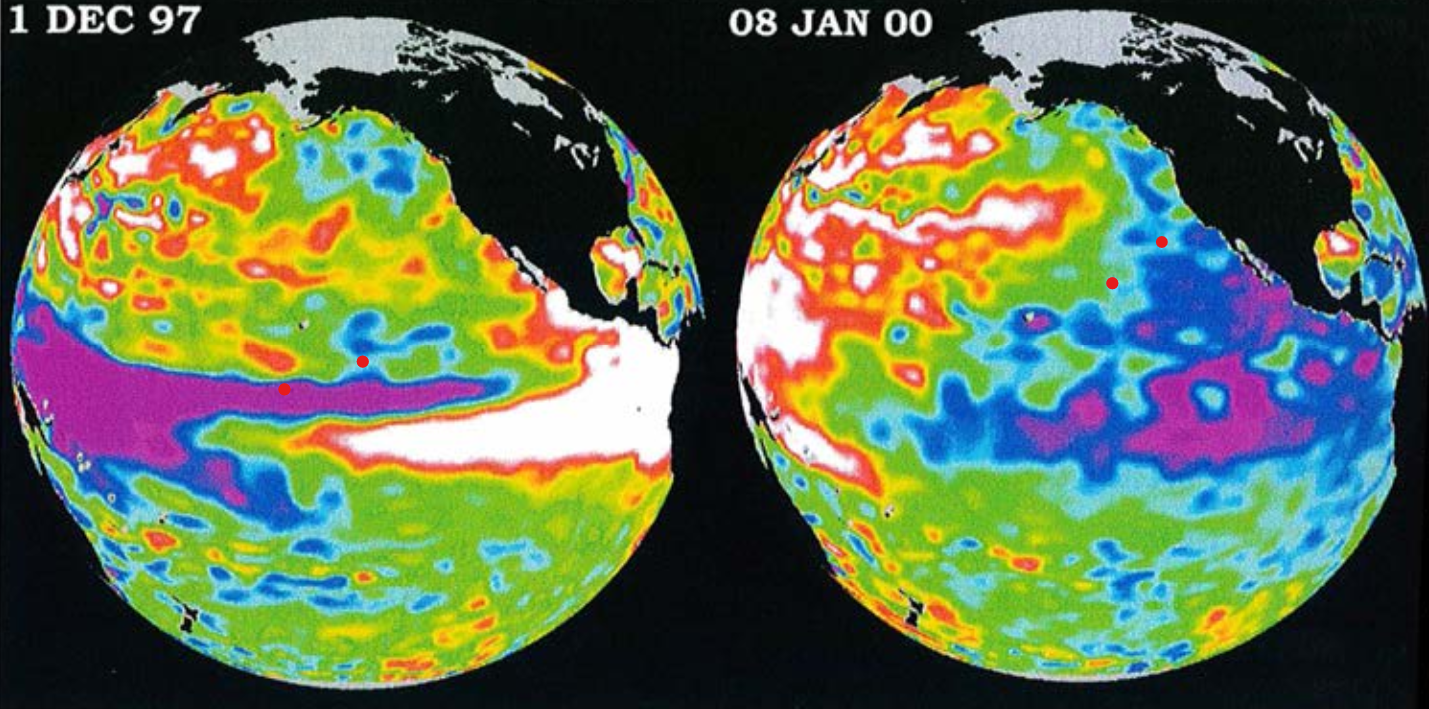
\includegraphics{2024-2025 Math 215 Assignments (in progress)/ENSO1.png}
    \caption{Temperature measurements illustrating the oscillation between El Ni\~no (left) and La Ni\~na (right) (Kapler and Engler, reprinted from NASA/JPL-Caltech)}
    \label{fig:enter-label}
\end{figure}


Note for instructors: Below we present two options for questions: one which contains all the parameters in the model and one which contains only one parameter. We present the questions using the full parameter set first. Note that for the questions with only one parameter, the rest of the parameter values are chosen so they line up with the computational part of the assignment. If the computational part of the assignment is not being used, simpler parameter values could be chosen.


%We proceed to approach solving this problem \textbf{with} and \textbf{without} the parameters. The solution gives the same behavior, but the parameter values line up with what is used computationally and make the process much simpler.

\section{Questions (including all parameters)}
The El Nino system can be represented by the following ODEs:
\begin{align}
    x' & = -x + \gamma (bx + y) - \varepsilon (bx + y)^3 \\
    y' & = -ry - \alpha  b x
\end{align}
where $x$ is proportional to the Sea Surface Temperature (SST) anomaly in the Eastern Pacific (the difference between the warm SST during El Nino and standard SST), and $y$ is  proportional to the thermocline depth anomaly in the Western Pacific.
\begin{enumerate}
    \item Linearize the system about the fixed point $(0,0)$ using the Jacobian. Find restrictions on the parameters so that solutions to the linearized system are purely oscillatory. Find the eigenvalues of the system in this case (they should be complex conjugates of each other and have zero real part). Hint: it might be useful to group $\gamma b = c$ once you linearize).

    \item When we observe pure oscillations, the solution set will have two complex conjugate eigenvalues $\lambda_1, \lambda_2 = \pm i\sqrt{\mathrm{Det}(A)}$. Find a general solution for this equation using the eigenvectors for these given eigenvalues. 


\end{enumerate}
\newpage





\section{Questions (with all but  one fixed parameter values)}
These two phenomena can be represented in a system of ODE's:
\begin{align}
    x' & = -x + \frac{3}{4} (bx + y) - 0.1(bx + y)^3 \\
    y' & = -\frac{1}{4}y -  \frac{b}{8} x
\end{align}
where $x$ is proportional to the Sea Surface Temperature (SST) anomaly in the Eastern Pacific (the difference between the warm SST during El Nino and standard SST), and $y$ is  proportional to the thermocline depth anomaly in the Western Pacific.
\begin{enumerate}
    \item  Linearize the system about the fixed point $(0,0)$ using the Jacobian. Find a restriction on the $b$ so that solutions to the linearized system are purely oscillatory. Find the eigenvalues of the system in this case (they should be complex conjugates of each other and have zero real part). Hint: once you find one restriction required for purely complex eigenvalues, use it to simplify the calculation of the eigenvalues.

    \item When we observe pure oscillations, the solution set will have two complex conjugate eigenvalues $\lambda_1, \lambda_2 = \pm i\sqrt{\mathrm{Det}(A)}$. Find a general solution for this equation using the eigenvectors for these given eigenvalues. Use the value of $b$ which you found in the previous problem. 


\end{enumerate}




\newpage

\section{Numerics assignment (for syzygy)}
(.ipynb file can be found in folder. If you make changes to ipynb file, you can run `jupyter nbconvert --to latex 215ENSOnumerics.ipynb' in the syzygy terminal to export assignment to latex)\\


    
    \hypertarget{enso-assignment}{%
\section*{ENSO assignment}\label{enso-assignment}}

The El Nino Southern Oscilllations are an observed phenomenon in which
the average tropical Eastern Pacific Sea Surface Temperature becomes
much colder than usual. This oscillation can be represented in a system
of two nonlinear ODE's, with the following two variables: \(x\) which is
proportional to the Sea Surface Temperature (SST) anomaly in the
tropical Eastern Pacific, and \(y\) which is proportional to the
thermocline depth anomaly in the Western Pacific. The thermocline is the
(rough) boundary between the warmer top layer of the ocean and the
cooler deep ocean layer.

    \hypertarget{consider-the-following-nonlinear-system-of-odes}{%
\section*{Consider the following nonlinear system of
ODEs:}\label{consider-the-following-nonlinear-system-of-odes}}

\begin{align}
    x' & = -x + \gamma (bx + y) - \varepsilon (bx + y)^3 \\
    y' & = -ry - \alpha b x
\end{align}

For this system, first find the linearization about the origin (by
hand), then follow the instructions on how to use plt.streamplot and
plot the linearization about the origin.

    These statements import the necessary tools to plot our equation:

    \begin{tcolorbox}[breakable, size=fbox, boxrule=1pt, pad at break*=1mm,colback=cellbackground, colframe=cellborder]
\prompt{In}{incolor}{5}{\boxspacing}
\begin{Verbatim}[commandchars=\\\{\}]
\PY{k+kn}{from} \PY{n+nn}{matplotlib}\PY{n+nn}{.}\PY{n+nn}{pyplot} \PY{k+kn}{import} \PY{n}{cm}
\PY{k+kn}{import} \PY{n+nn}{matplotlib}\PY{n+nn}{.}\PY{n+nn}{pyplot} \PY{k}{as} \PY{n+nn}{plt}
\PY{k+kn}{import} \PY{n+nn}{numpy} \PY{k}{as} \PY{n+nn}{np}
\PY{k+kn}{import} \PY{n+nn}{math}
\end{Verbatim}
\end{tcolorbox}

    The constants below determine the behavior of the system around the
origin. Feel free to change these parameters and see what happens to the
linearization.

    \begin{tcolorbox}[breakable, size=fbox, boxrule=1pt, pad at break*=1mm,colback=cellbackground, colframe=cellborder]
\prompt{In}{incolor}{6}{\boxspacing}
\begin{Verbatim}[commandchars=\\\{\}]
\PY{n}{g} \PY{o}{=} \PY{l+m+mi}{3}\PY{o}{/}\PY{l+m+mi}{4} \PY{c+c1}{\PYZsh{}gamma}
\PY{n}{b} \PY{o}{=} \PY{l+m+mi}{5}\PY{o}{/}\PY{l+m+mi}{3}
\PY{n}{e} \PY{o}{=} \PY{l+m+mf}{0.1} \PY{c+c1}{\PYZsh{}epsilon}
\PY{n}{r} \PY{o}{=} \PY{l+m+mi}{1}\PY{o}{/}\PY{l+m+mi}{4}
\PY{n}{a} \PY{o}{=} \PY{l+m+mi}{1}\PY{o}{/}\PY{l+m+mi}{8} \PY{c+c1}{\PYZsh{}alpha}
\end{Verbatim}
\end{tcolorbox}

    The following code segment sets up a meshgrid (i.e.~small rectangular
chunks that we can solve the equation in) The bounds in np.arrange
describe the size of the meshgrid, or the domain over which we're
solving.

    \begin{tcolorbox}[breakable, size=fbox, boxrule=1pt, pad at break*=1mm,colback=cellbackground, colframe=cellborder]
\prompt{In}{incolor}{7}{\boxspacing}
\begin{Verbatim}[commandchars=\\\{\}]
\PY{n}{nx}\PY{p}{,} \PY{n}{ny} \PY{o}{=} \PY{l+m+mf}{.1}\PY{p}{,} \PY{l+m+mf}{.1}
\PY{n}{x} \PY{o}{=} \PY{n}{np}\PY{o}{.}\PY{n}{arange}\PY{p}{(}\PY{o}{\PYZhy{}}\PY{l+m+mi}{2}\PY{p}{,} \PY{l+m+mi}{2}\PY{p}{,} \PY{n}{nx}\PY{p}{)}
\PY{n}{y} \PY{o}{=} \PY{n}{np}\PY{o}{.}\PY{n}{arange}\PY{p}{(}\PY{o}{\PYZhy{}}\PY{l+m+mi}{2}\PY{p}{,} \PY{l+m+mi}{2}\PY{p}{,} \PY{n}{ny}\PY{p}{)}
\PY{n}{X}\PY{p}{,} \PY{n}{Y} \PY{o}{=} \PY{n}{np}\PY{o}{.}\PY{n}{meshgrid}\PY{p}{(}\PY{n}{x}\PY{p}{,} \PY{n}{y}\PY{p}{)}
\end{Verbatim}
\end{tcolorbox}

    Next, add your linearized system below: e.g.~

dx = -x + \ldots{}

dy = -r*y -\ldots{}

    \begin{tcolorbox}[breakable, size=fbox, boxrule=1pt, pad at break*=1mm,colback=cellbackground, colframe=cellborder]
\prompt{In}{incolor}{4}{\boxspacing}
\begin{Verbatim}[commandchars=\\\{\}]
\PY{n}{dx} \PY{o}{=} 
\PY{n}{dy} \PY{o}{=} 
\end{Verbatim}
\end{tcolorbox}



    The block below plots the system for the given differential equations
using different points on the meshgrid as initial conditions to
computationally solve the system. This is essentially a slope field, but
with more connected trajectories. Use the information provided
\href{https://matplotlib.org/stable/api/_as_gen/matplotlib.pyplot.streamplot.html}{here}
to run the command plt.streamplot.

    \begin{tcolorbox}[breakable, size=fbox, boxrule=1pt, pad at break*=1mm,colback=cellbackground, colframe=cellborder]
\prompt{In}{incolor}{ }{\boxspacing}
\begin{Verbatim}[commandchars=\\\{\}]
\PY{n}{plt}\PY{o}{.}\PY{n}{streamplot}\PY{p}{(}\PY{n}{X}\PY{p}{,}\PY{n}{Y}\PY{p}{,}\PY{n}{dx}\PY{p}{,} \PY{n}{dy}\PY{p}{,} \PY{n}{density}\PY{o}{=}\PY{l+m+mi}{2}\PY{p}{,} \PY{n}{cmap}\PY{o}{=} \PY{l+s+s1}{\PYZsq{}}\PY{l+s+s1}{jet}\PY{l+s+s1}{\PYZsq{}}\PY{p}{,} \PY{n}{arrowsize}\PY{o}{=}\PY{l+m+mi}{1}\PY{p}{)}
\end{Verbatim}
\end{tcolorbox}

    

    Now add your solution to the linearized system from the written
assignment to the code block below. When you run the code block, your
solution will be overlaid overtop the slope field. Modify \(c_1\) and
\(c_2\) so that the range of your solution in \(x\) is approximately
between -0.5 and 0.5. Because you are not required to start at a
specific initial condition, you may set one of your constants to zero
and only modify the other constant. Keep the parameters constant at this
point onwards.

    \begin{tcolorbox}[breakable, size=fbox, boxrule=1pt, pad at break*=1mm,colback=cellbackground, colframe=cellborder]
\prompt{In}{incolor}{ }{\boxspacing}
\begin{Verbatim}[commandchars=\\\{\}]
\PY{c+c1}{\PYZsh{}Note: use np.cos(t) for cos(t), np.sin(t) for sin(t), and np.sqrt() to sqrt()}
\PY{c+c1}{\PYZsh{} use x**2 to enter x\PYZca{}2}
\PY{n}{g} \PY{o}{=} \PY{l+m+mi}{3}\PY{o}{/}\PY{l+m+mi}{4} \PY{c+c1}{\PYZsh{}gamma}
\PY{n}{b} \PY{o}{=} \PY{l+m+mi}{5}\PY{o}{/}\PY{l+m+mi}{3}
\PY{n}{e} \PY{o}{=} \PY{l+m+mf}{0.1} \PY{c+c1}{\PYZsh{}epsilon}
\PY{n}{r} \PY{o}{=} \PY{l+m+mi}{1}\PY{o}{/}\PY{l+m+mi}{4}
\PY{n}{a} \PY{o}{=} \PY{l+m+mi}{1}\PY{o}{/}\PY{l+m+mi}{8} \PY{c+c1}{\PYZsh{}alpha}

\PY{n}{c\PYZus{}1} \PY{o}{=} 
\PY{n}{c\PYZus{}2} \PY{o}{=} 

\PY{n}{w\PYZus{}c} \PY{o}{=} \PY{c+c1}{\PYZsh{}you can define omega here in terms of the other parameters if you\PYZsq{}d like, it may make it easier to enter your solution}

\PY{n}{t}\PY{o}{=}\PY{n}{np}\PY{o}{.}\PY{n}{linspace}\PY{p}{(}\PY{l+m+mi}{0}\PY{p}{,}\PY{l+m+mi}{50}\PY{p}{,}\PY{l+m+mi}{100}\PY{p}{)}

\PY{k}{def} \PY{n+nf}{x}\PY{p}{(}\PY{n}{t}\PY{p}{)}\PY{p}{:}
    \PY{k}{return} \PY{c+c1}{\PYZsh{}add your function before this comment}

\PY{k}{def} \PY{n+nf}{y}\PY{p}{(}\PY{n}{t}\PY{p}{)}\PY{p}{:}
    \PY{k}{return} \PY{c+c1}{\PYZsh{}add your function before this comment}

\PY{n}{plt}\PY{o}{.}\PY{n}{streamplot}\PY{p}{(}\PY{n}{X}\PY{p}{,}\PY{n}{Y}\PY{p}{,}\PY{n}{dx}\PY{p}{,} \PY{n}{dy}\PY{p}{,} \PY{n}{density}\PY{o}{=}\PY{l+m+mi}{2}\PY{p}{,} \PY{n}{cmap}\PY{o}{=} \PY{l+s+s1}{\PYZsq{}}\PY{l+s+s1}{jet}\PY{l+s+s1}{\PYZsq{}}\PY{p}{,} \PY{n}{arrowsize}\PY{o}{=}\PY{l+m+mi}{1}\PY{p}{)}
\PY{n}{plt}\PY{o}{.}\PY{n}{plot}\PY{p}{(}\PY{n}{x}\PY{p}{(}\PY{n}{t}\PY{p}{)}\PY{p}{,}\PY{n}{y}\PY{p}{(}\PY{n}{t}\PY{p}{)}\PY{p}{)}
\end{Verbatim}
\end{tcolorbox}


    


The code below plots the slope field for the full non-linear system and
overlays your linearized solution on top. It also plots one trajectory
of the numerical solution to the non-linear equation so that you can see
how well the non-linear solution aligns with your linearized solution.

What you see is the existence of a stable limit cycle in the non-linear
system, this means that all trajectories approach the cycle that is
approximated by your linearized solution.

Note: You can go back to the code box above and edit your \(c_1\) and
\(c_2\) if you want to change the amplitude of your linearized solution
so that it lines up well with the numerical solution to the non-linear
system.

    \begin{tcolorbox}[breakable, size=fbox, boxrule=1pt, pad at break*=1mm,colback=cellbackground, colframe=cellborder]
\prompt{In}{incolor}{10}{\boxspacing}
\begin{Verbatim}[commandchars=\\\{\}]
\PY{c+c1}{\PYZsh{}First, find numerical solution to full non\PYZhy{}linear system}
\PY{c+c1}{\PYZsh{}Set b=5.3/3. This is because at b=5/3 the fixed point is actually stable, so we need to increase b a little to generate a limit cycle that will match with the linearized solution}
\PY{n}{b}\PY{o}{=}\PY{l+m+mf}{5.3}\PY{o}{/}\PY{l+m+mi}{3}
\PY{k+kn}{from} \PY{n+nn}{scipy}\PY{n+nn}{.}\PY{n+nn}{integrate} \PY{k+kn}{import} \PY{n}{solve\PYZus{}ivp}
\PY{k}{def} \PY{n+nf}{thc}\PY{p}{(}\PY{n}{t}\PY{p}{,}\PY{n}{z}\PY{p}{,}\PY{n}{a}\PY{p}{,}\PY{n}{b}\PY{p}{,}\PY{n}{e}\PY{p}{,}\PY{n}{g}\PY{p}{,}\PY{n}{r}\PY{p}{)}\PY{p}{:}
    \PY{n}{x}\PY{p}{,}\PY{n}{y}\PY{o}{=}\PY{n}{z}
    \PY{k}{return} \PY{p}{[}\PY{o}{\PYZhy{}}\PY{n}{x} \PY{o}{+} \PY{n}{g}\PY{o}{*}\PY{p}{(}\PY{n}{b}\PY{o}{*}\PY{n}{x} \PY{o}{+} \PY{n}{y}\PY{p}{)} \PY{o}{\PYZhy{}} \PY{n}{e}\PY{o}{*}\PY{p}{(}\PY{n}{b}\PY{o}{*}\PY{n}{x} \PY{o}{+} \PY{n}{y}\PY{p}{)}\PY{o}{*}\PY{o}{*}\PY{l+m+mi}{3}\PY{p}{,} \PY{o}{\PYZhy{}}\PY{n}{r}\PY{o}{*}\PY{n}{y} \PY{o}{\PYZhy{}} \PY{n}{a}\PY{o}{*}\PY{n}{b}\PY{o}{*}\PY{n}{x}\PY{p}{]}

\PY{n}{t\PYZus{}eval} \PY{o}{=} \PY{n}{np}\PY{o}{.}\PY{n}{linspace}\PY{p}{(}\PY{l+m+mi}{0}\PY{p}{,}\PY{l+m+mi}{100}\PY{p}{,}\PY{l+m+mi}{500}\PY{p}{)}

\PY{c+c1}{\PYZsh{} Here the [1,1] part of the code specifies the initial conditions. Feel free to change them}
\PY{n}{sol} \PY{o}{=} \PY{n}{solve\PYZus{}ivp}\PY{p}{(}\PY{n}{thc}\PY{p}{,} \PY{p}{[}\PY{l+m+mi}{0}\PY{p}{,} \PY{l+m+mi}{100}\PY{p}{]}\PY{p}{,} \PY{p}{[}\PY{l+m+mi}{1}\PY{p}{,} \PY{l+m+mi}{1}\PY{p}{]}\PY{p}{,} \PY{n}{t\PYZus{}eval}\PY{o}{=}\PY{n}{t\PYZus{}eval}\PY{p}{,} \PY{n}{args}\PY{o}{=}\PY{p}{(}\PY{n}{a}\PY{p}{,}\PY{n}{b}\PY{p}{,}\PY{n}{e}\PY{p}{,}\PY{n}{g}\PY{p}{,}\PY{n}{r}\PY{p}{)}\PY{p}{,} \PY{n}{max\PYZus{}step}\PY{o}{=}\PY{l+m+mf}{0.01}\PY{p}{)}

\PY{c+c1}{\PYZsh{}plot slopefield:}
\PY{n}{dx} \PY{o}{=} \PY{o}{\PYZhy{}}\PY{n}{X} \PY{o}{+} \PY{n}{g}\PY{o}{*}\PY{p}{(}\PY{n}{b}\PY{o}{*}\PY{n}{X} \PY{o}{+} \PY{n}{Y}\PY{p}{)} \PY{o}{\PYZhy{}} \PY{n}{e}\PY{o}{*}\PY{p}{(}\PY{n}{b}\PY{o}{*}\PY{n}{X} \PY{o}{+} \PY{n}{Y}\PY{p}{)}\PY{o}{*}\PY{o}{*}\PY{l+m+mi}{3}
\PY{n}{dy} \PY{o}{=} \PY{o}{\PYZhy{}}\PY{n}{r}\PY{o}{*}\PY{n}{Y} \PY{o}{\PYZhy{}} \PY{n}{a}\PY{o}{*}\PY{n}{b}\PY{o}{*}\PY{n}{X}
\PY{n}{plt}\PY{o}{.}\PY{n}{streamplot}\PY{p}{(}\PY{n}{X}\PY{p}{,}\PY{n}{Y}\PY{p}{,}\PY{n}{dx}\PY{p}{,} \PY{n}{dy}\PY{p}{,} \PY{n}{density}\PY{o}{=}\PY{l+m+mi}{2}\PY{p}{,} \PY{n}{cmap}\PY{o}{=} \PY{l+s+s1}{\PYZsq{}}\PY{l+s+s1}{jet}\PY{l+s+s1}{\PYZsq{}}\PY{p}{,} \PY{n}{arrowsize}\PY{o}{=}\PY{l+m+mi}{1}\PY{p}{)}

\PY{c+c1}{\PYZsh{}plot numerical solution:}
\PY{n}{plt}\PY{o}{.}\PY{n}{plot}\PY{p}{(}\PY{n}{sol}\PY{o}{.}\PY{n}{y}\PY{o}{.}\PY{n}{T}\PY{p}{[}\PY{p}{:}\PY{p}{,} \PY{l+m+mi}{0}\PY{p}{]}\PY{p}{,} \PY{n}{sol}\PY{o}{.}\PY{n}{y}\PY{o}{.}\PY{n}{T}\PY{p}{[}\PY{p}{:}\PY{p}{,} \PY{l+m+mi}{1}\PY{p}{]}\PY{p}{)}

\PY{c+c1}{\PYZsh{}plot your linearized solution:}
\PY{n}{plt}\PY{o}{.}\PY{n}{plot}\PY{p}{(}\PY{n}{x}\PY{p}{(}\PY{n}{t}\PY{p}{)}\PY{p}{,}\PY{n}{y}\PY{p}{(}\PY{n}{t}\PY{p}{)}\PY{p}{)}
\end{Verbatim}
\end{tcolorbox}



     





\newpage
\section{Additional Information}
 The system setup here follows from a process called \textit{nondimensionalization}, where constants are divided through and lumped into new, dimensionless variables. The original system for ENSO follows:
 \begin{align}
    \dfrac{dT_E}{dt} =& -cT_E + \gamma'(h_w + b'T_E) - \epsilon'(h_w + b'T_E)^3\\
    \dfrac{dh_w}{dt} =& -r'h_w -\alpha' b' T_E
 \end{align}
Where $T_E$ is the average sea surface temperature in the eastern pacific, and $h_w$ is the thermocline depth anomaly in the western pacific. The thermocline depth describes the boundary between the warmer, top layer of the ocean and the cooler layer below it. The rest of the constants are positive.\\
Next, we can follow the process of nondimensionalization. There are two reference parameters, $T_0$ and $h_0$ - the standard eastern ocean temperature and western thermocline depth. 

\begin{tabular}{ |p{3cm}|p{3cm}| }
\hline
\multicolumn{2}{|c|}{Variable definitions} \\
\hline
Variable & Value in terms of ODE\\
\hline
$x$ & $\dfrac{T_E}{T_0}$  \\
$y$ & $\dfrac{h_w}{h_0}$ \\
$\tau$ &  $ct$ \\
$r$ & $\dfrac{r'}{c}$  \\
$\alpha$ & $\dfrac{\alpha'}{c}$ \\
$\gamma$ & $\dfrac{h_0\gamma'}{T_0c}$   \\
$b$ & $\dfrac{T_0}{h_0}b'$  \\
$\epsilon$ & $\dfrac{h_0^3}{T_0c}\epsilon'$ \\
\hline
\end{tabular} \\

Generally, $h_0 = 150 m$, $T_0 = 7.5 K$, and $c= 2$ months. 
For the equations below, $\dot x=\frac{dx}{d\tau}$. This gives us the original system mentioned in $(1)$ and $(2)$:
\begin{align}
    \dot x & = -x + \gamma (bx + y) - \varepsilon (bx + y)^3 \\
    \dot y & = -ry - \alpha b x
\end{align}

%Also, $\tau$ will still be a derivative in time - just scaled by $c$. This means we can still phrase the question in terms of a time derivative. 

\begin{thebibliography}{9}
\bibitem{figure}
Kaper, H. G, and Hans Engler. \emph{Mathematics and Climate}. Philadelphia, Pennsylvania: Society for Industrial and Applied Mathematics SIAM, 3600 Market Street, Floor 6, Philadelphia, PA 19104, 2013. Print.
\end{thebibliography}

\end{document}